\section{Systematic Uncertainties}
\label{sec:syst}

%Systematics: main systematics should be available

%-----------------------------------------------------
%\subsection{Background Modeling Uncertainties} 
%\label{sec:syst_bkg}
%
%Two sources of uncertainty on the background are assessed and incorporated in the fits: spurious signal and ML modeling. 
%
%
%%TODO: The alternate polynomial uncertainty is assessed by fitting higher-order polynomials to the \mt~spectra.
%
%The ML modeling uncertainty is assessed by training the PFN over an alternate source of training events, namely the ``representative" MC background consisting of all backgrounds (eg. including top, V+jets, etc.) rather than just training on QCD. 


%-----------------------------------------------------
%\subsection{Signal Uncertainties} 
%\label{sec:syst_sig}

As it is typically done in dijet resonance searches using a polynomial fit, the systematic uncertainties in this analysis are applied only to the signal and not to the background. 
Any non-resonant variation on the \mt~spectrum itself is absorbed by the background fit and the impact on the residuals is expected to be small.


\subsection{Flat Uncertainties}
The standard flat uncertainty of 0.83\% will be applied to all signals for the luminosity uncertainty (1.13\%, 0.89\%, 1.13\%, and 1.10\% in 2015, 2016, 2017, and 2018 respectively), as described in Ref.~\cite{ATLAS-CONF-2019-021}.

%------------------------------------------------------------
\subsection{Spurious Signal}

Figure~\ref{fig:splusb_ex} shows some examples of S+B fits on the background-only distribution for a variety of signal hypotheses across the (\rinv, mass) grid.
\begin{figure}[!htbp]
\centering
   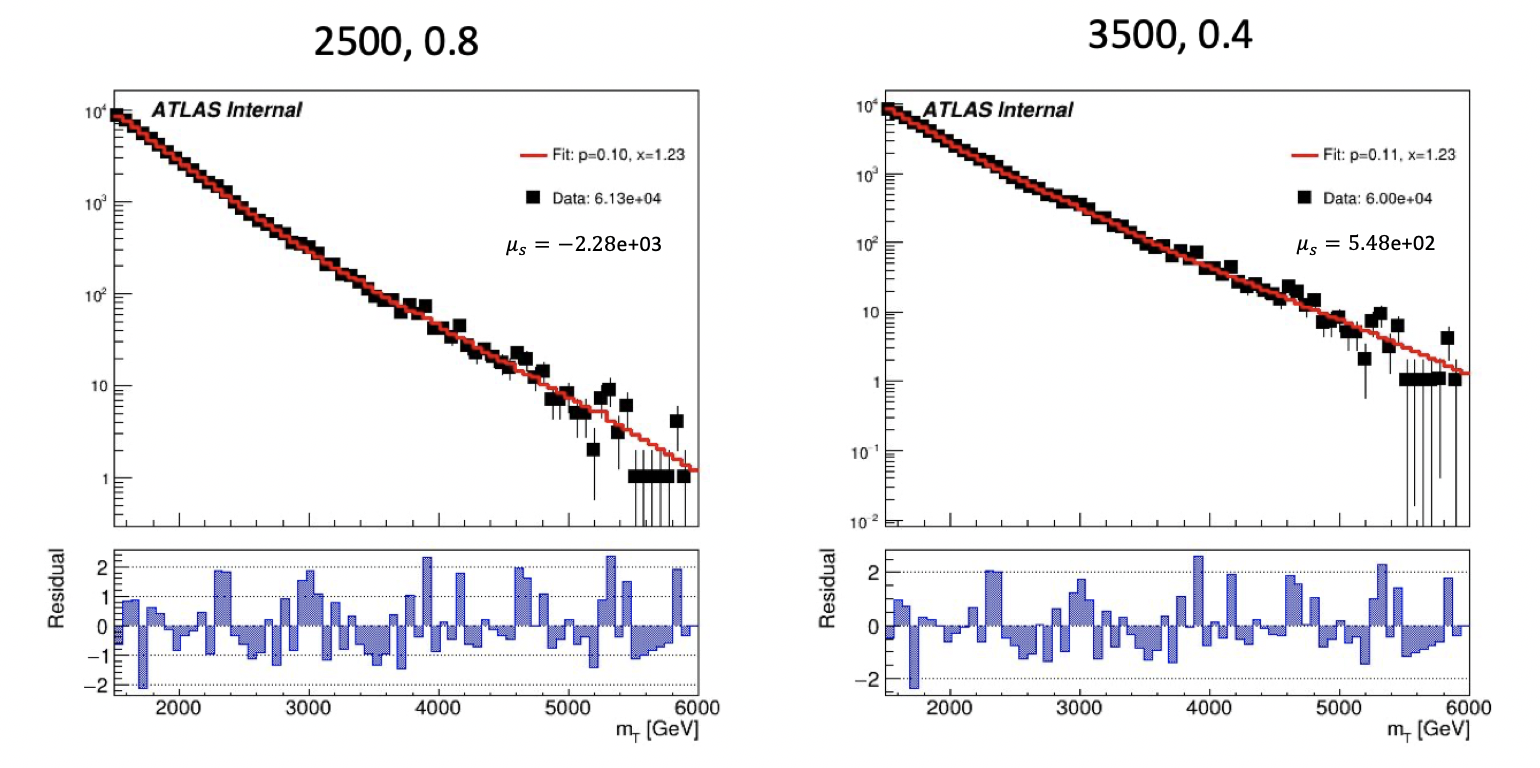
\includegraphics[width=0.8\textwidth]{figures/stats/splusb_ex1}
   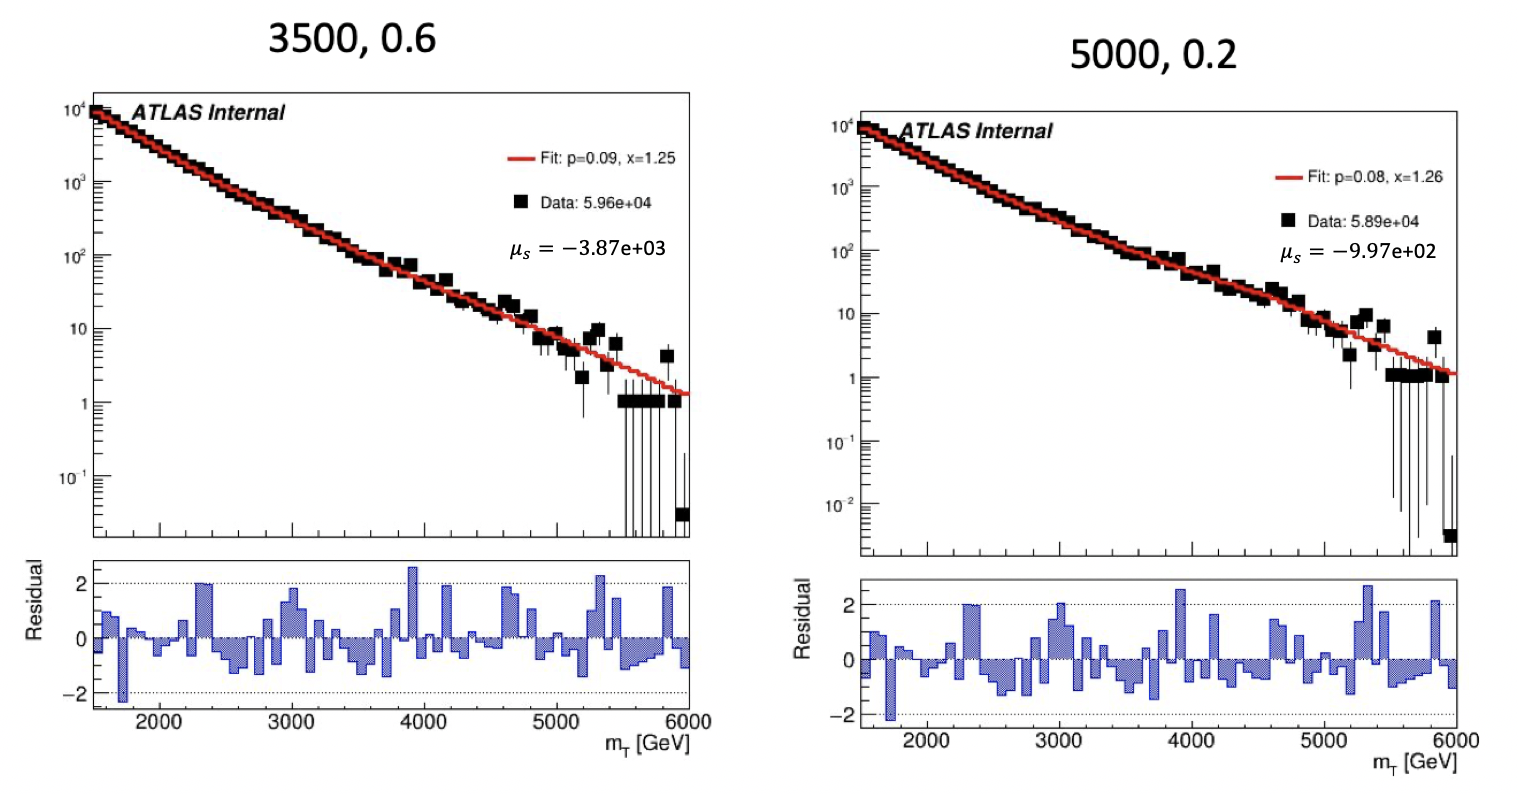
\includegraphics[width=0.8\textwidth]{figures/stats/splusb_ex2}
    \caption{Example S+B fits on background only spectrum (without systematics) for a variety of signal points.
    \label{fig:splusb_ex}}
\end{figure}


The spurious signal uncertainty is assessed following the prescription in Ref.~\cite{ATL-PHYS-PUB-2020-028} for the modeling of smooth backgrounds.
In this procedure, the spurious signal is defined using pseudo-data experiments, which are drawn from a smoothed template as described in Section~\ref{sec:stat}, from the CR \mt~shape.
It is included in the statistical treatment as a \textit{yield} uncertainty on each signal point in S+B fits.

The spurious signal is quantified for each signal as the mean number of signal events fitted in a signal-free spectrum (S$_{\text{spur}}$) divided by the RMS of the fitted spurious signal distribution $\sigma_{\text{fit}}$, considering many pseudo-data experiments.
Figure~\ref{fig:spursig_ex} gives examples of these pseudo-data experiments, revealing Gaussian distributions from which the mean is ascribed to the fitted spurious signal.
%Figure~\ref{fig:spursig_nevents} shows the determined spurious signal as a function of Z' resonance mass, for both low and high \rinv~points.
Figure~\ref{fig:spursig} shows the fitted spurious signal in terms of significance, calculated from the number of fitted events divided by the uncertainty (considered as the RMS of the distribution of spurious signal trials).
The measured S$_{spur}$ is generally below 0.5$\sigma$ across the grid, as recommended. 
The fraction of S+B fits that succeed in the CR are shown in Figure~\ref{fig:spursig_success}.
\begin{figure}[!htbp]
\centering
   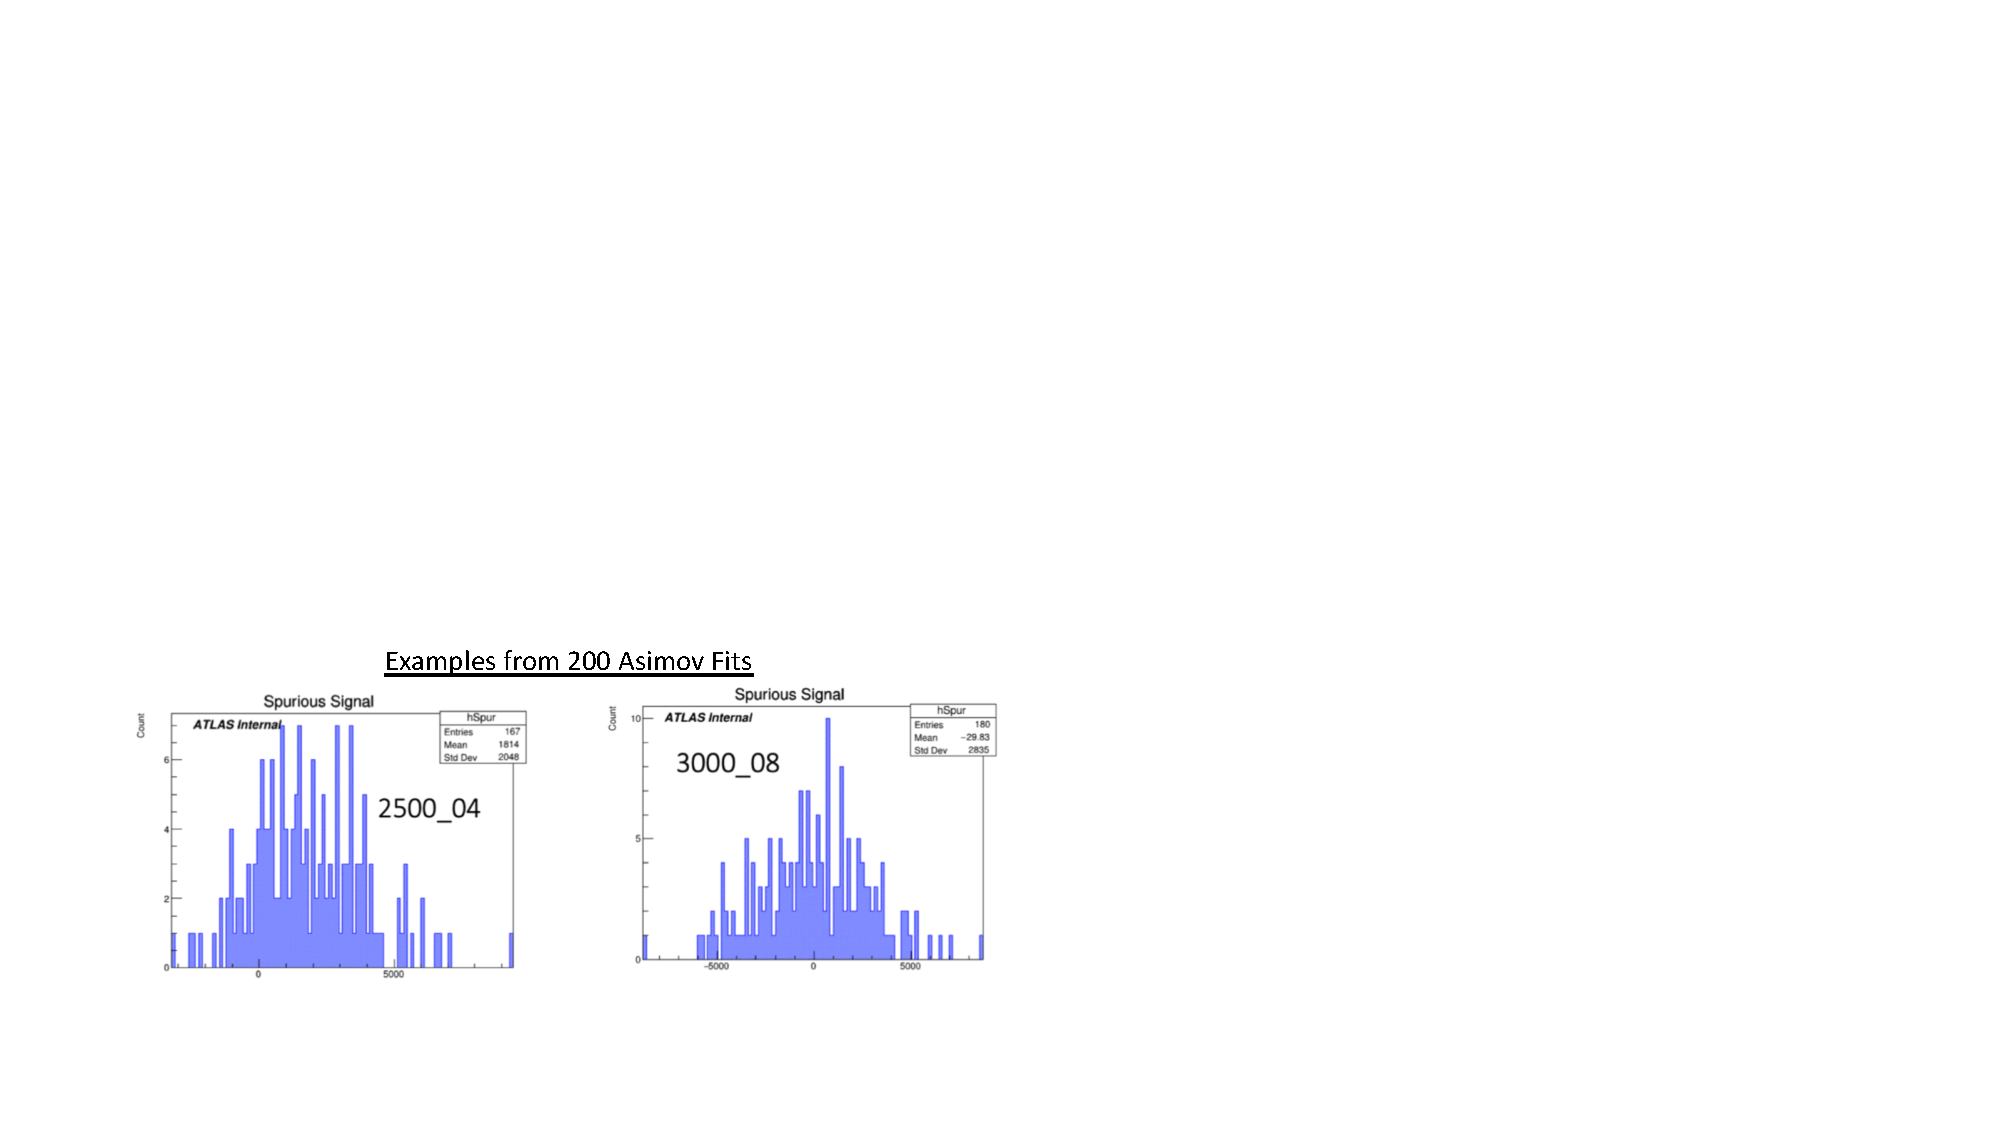
\includegraphics[width=0.8\textwidth]{figures/systs/spursig_ex}
    \caption{Example spurious signal fits, indicating a Gaussian distribution around the mean of spurious signal events.
    \label{fig:spursig_ex}}
\end{figure}
\begin{figure}[!htbp]
\centering
   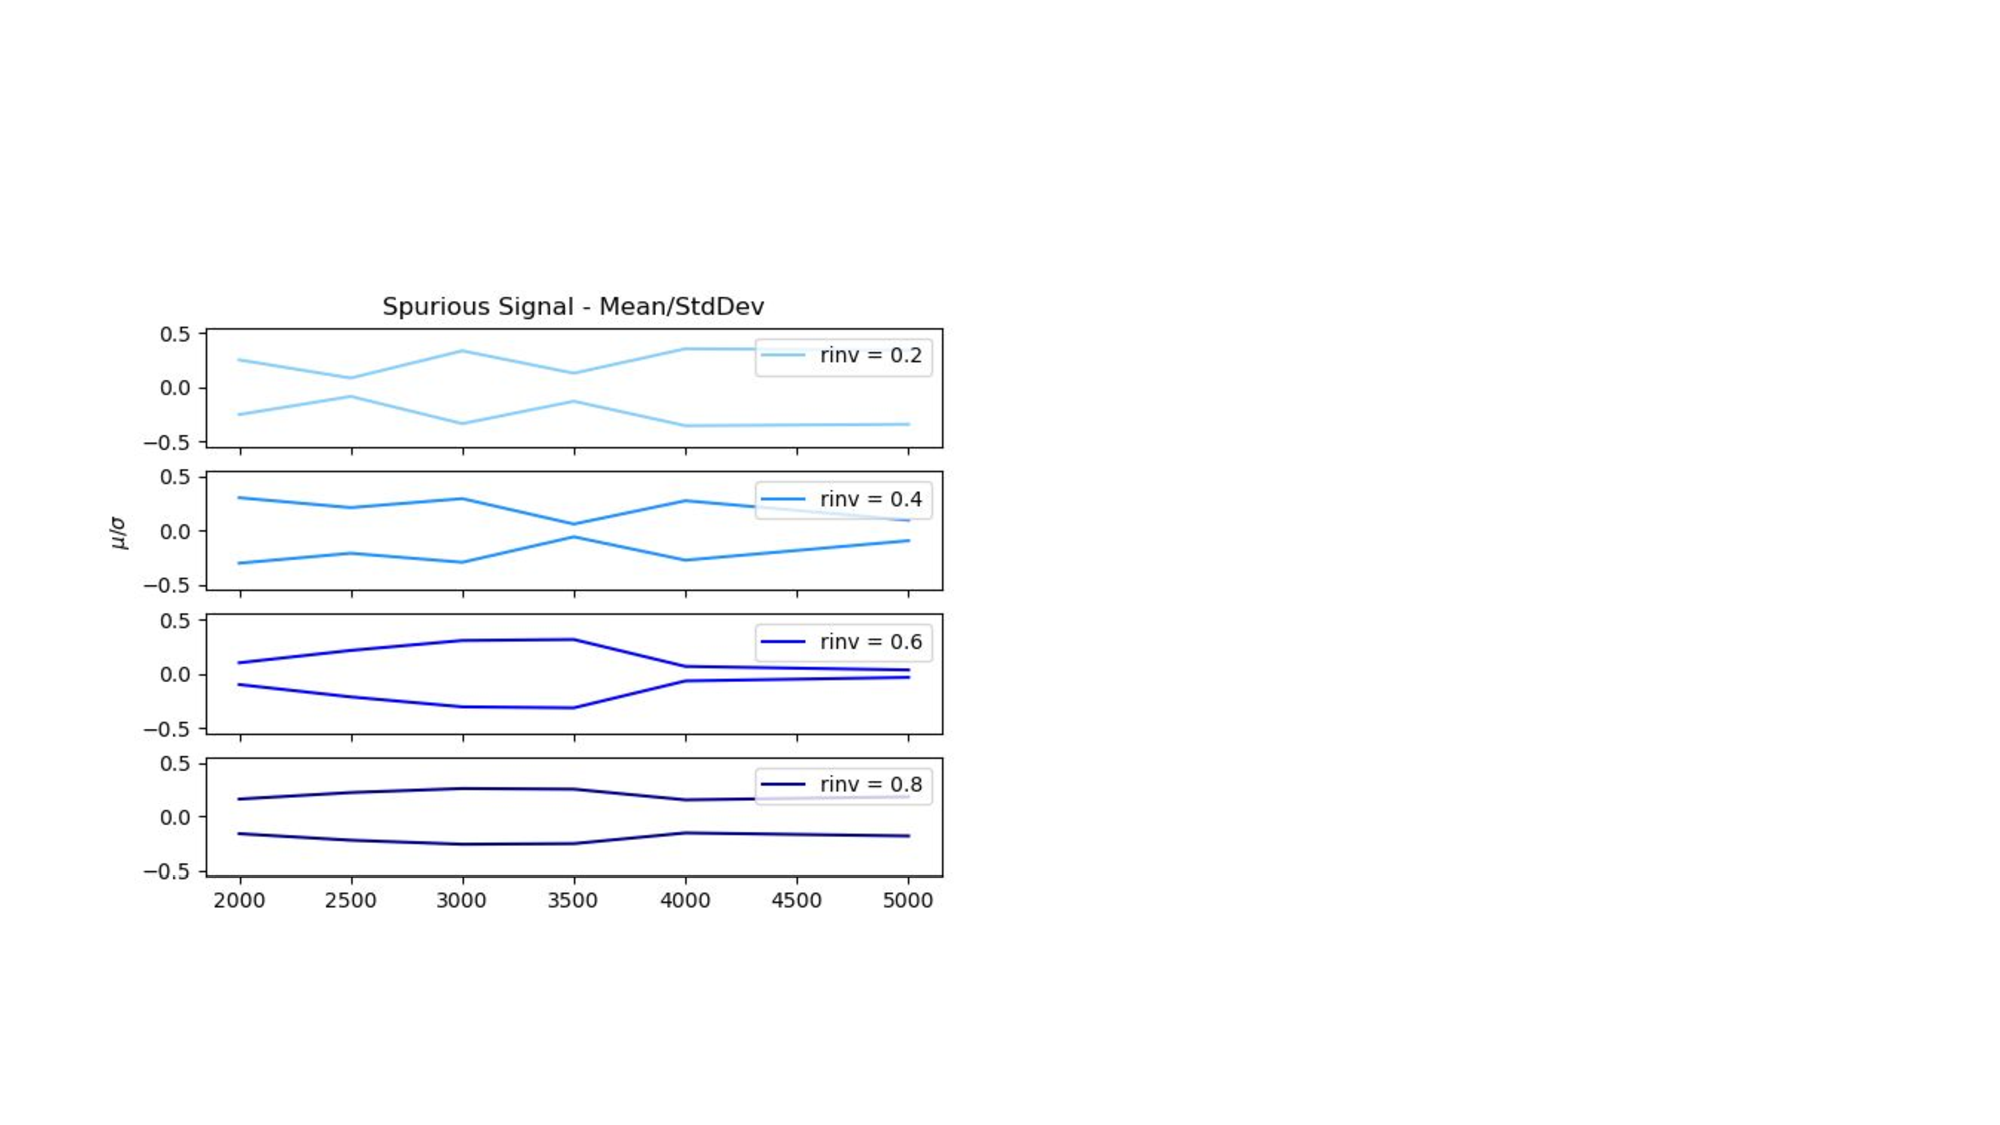
\includegraphics[width=0.6\textwidth]{figures/systs/spursig}
    \caption{Spurious signal, quantified as a number of fitted signal events divided by fit error in the CR, as a function of resonance mass.
    \label{fig:spursig}}
\end{figure}
\begin{figure}[!htbp]
\centering
   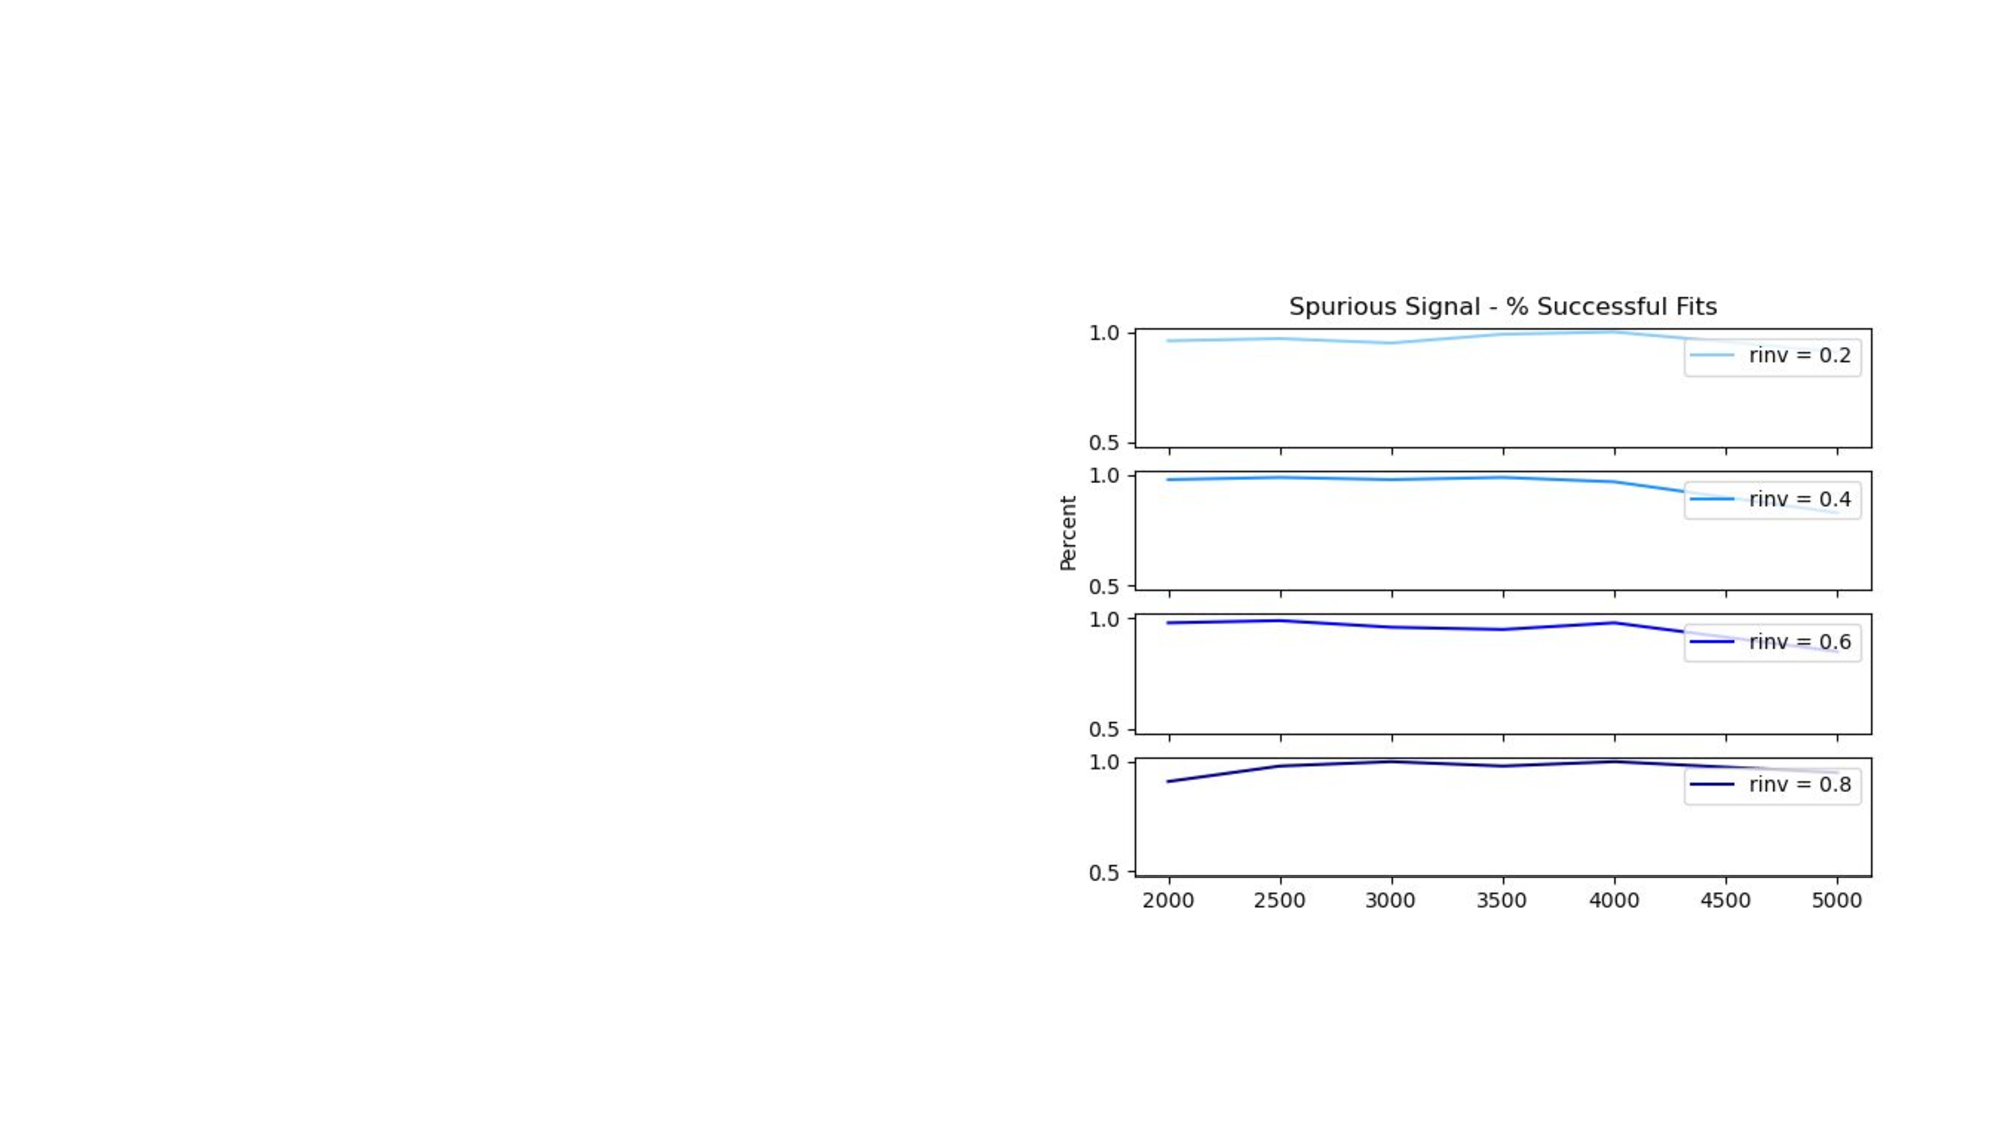
\includegraphics[width=0.6\textwidth]{figures/systs/spursig_success_cr}
   %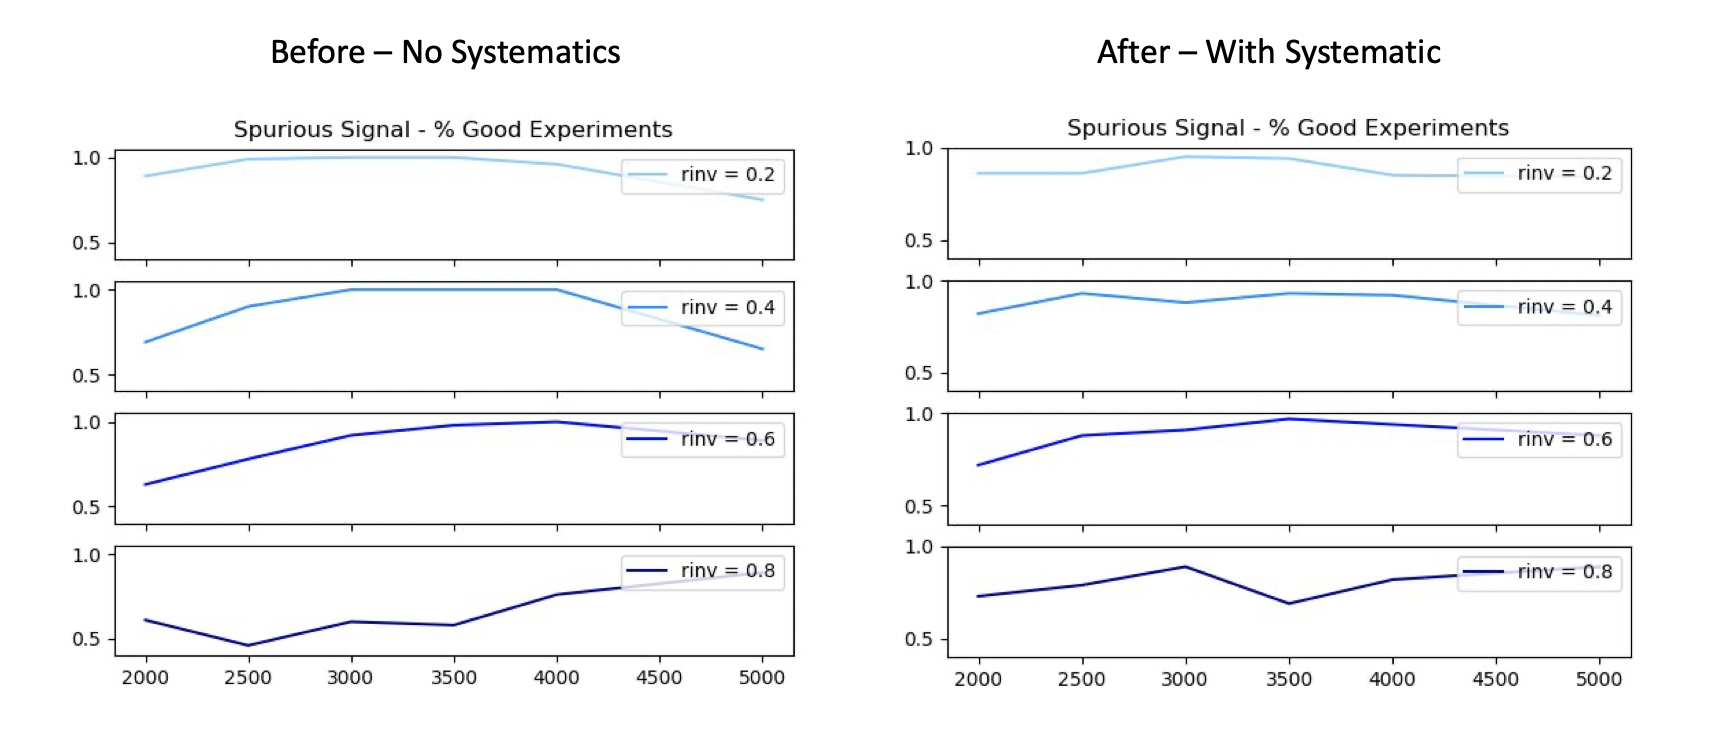
\includegraphics[width=0.95\textwidth]{figures/systs/spursig_success}
    \caption{Fraction of Asimov fits that succeed in the CR.
    \label{fig:spursig_success}}
\end{figure}

The effect of the spurious signal uncertainty is tested by considering the fitted spurious signal before and after the addition of the yield uncertainty.
This is done in Asimov data to give many trials.
Further, the addition of the spurious signal uncertainty minimally impacts the amount of signal that can be fit, as can be shown in the right side of Figure~\ref{fig:spursig_beforeafter}.
\begin{figure}[!htbp]
\centering
   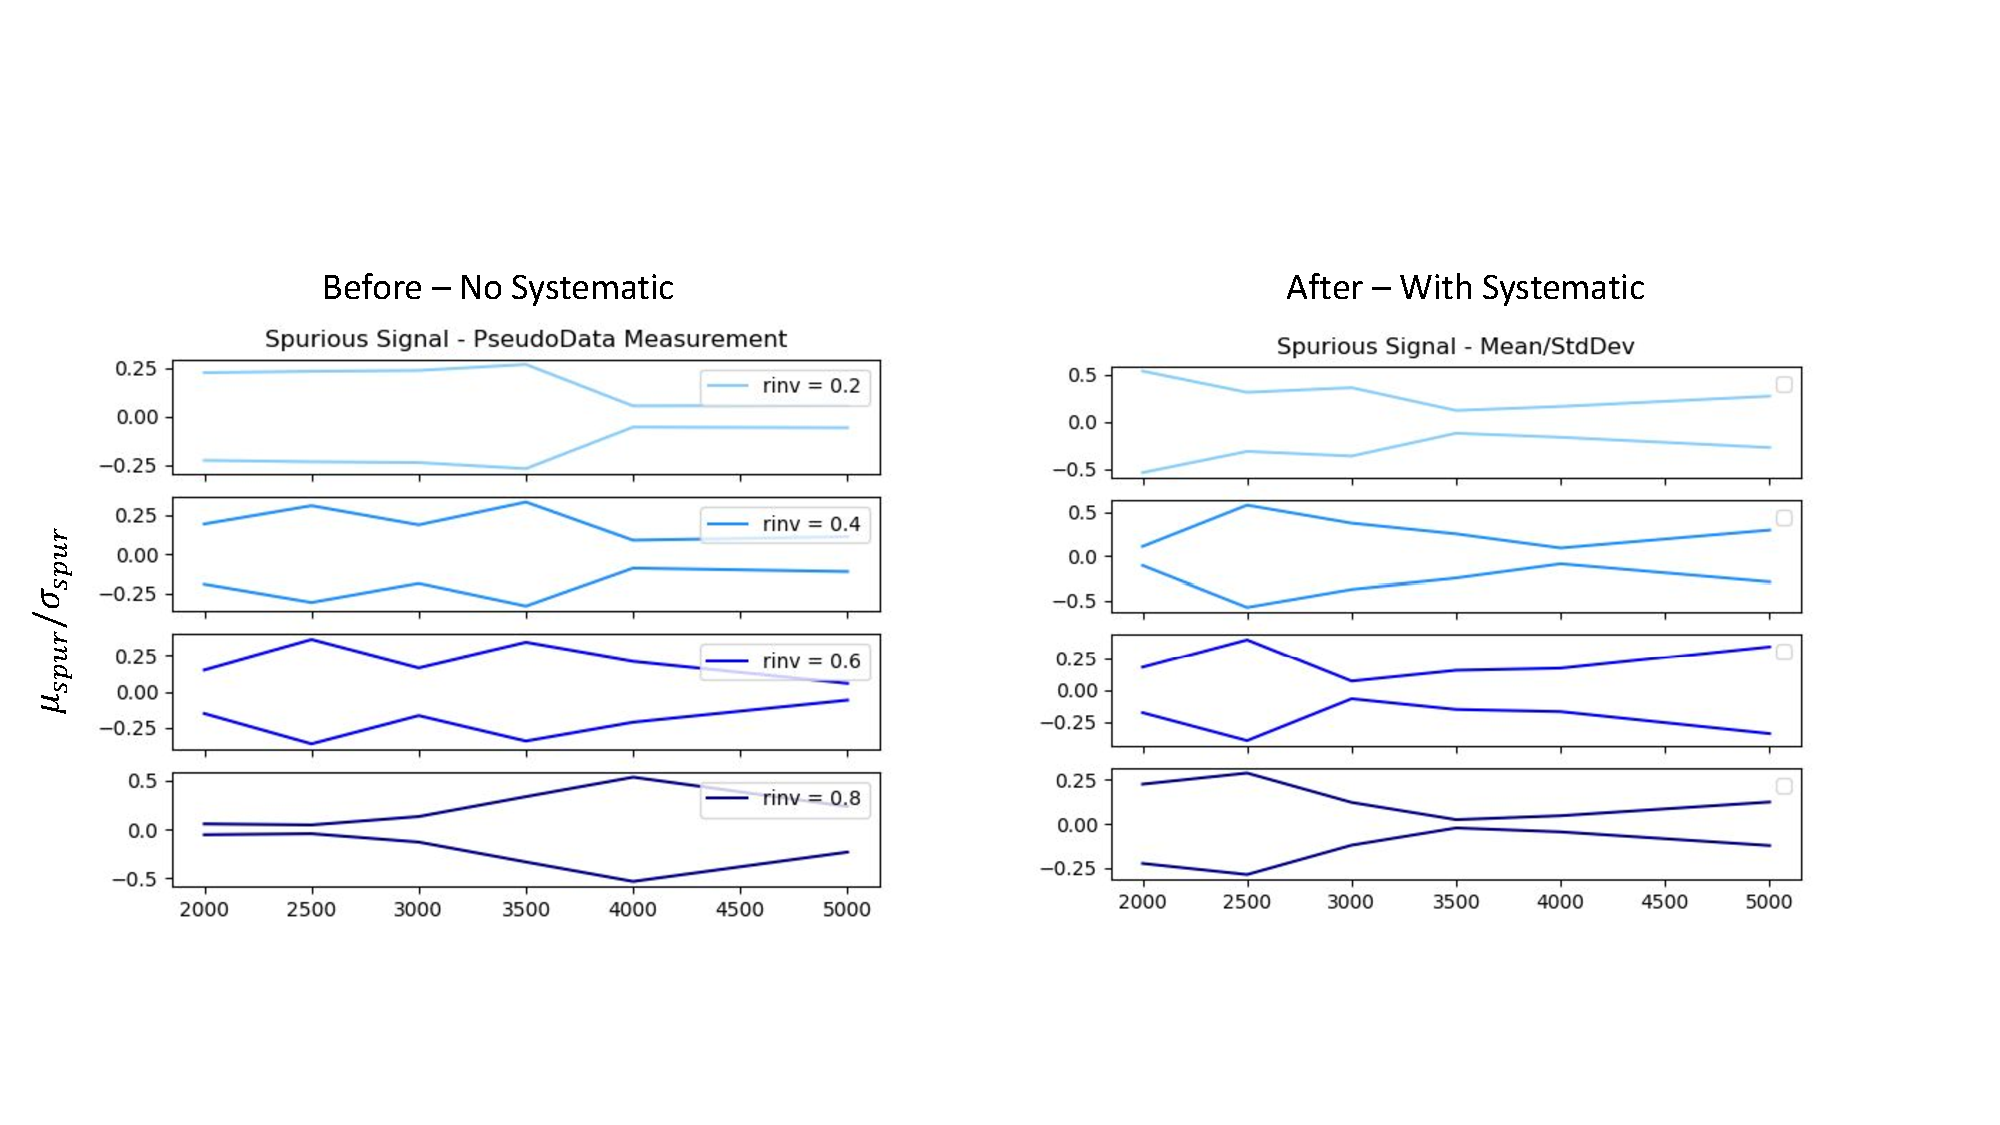
\includegraphics[width=0.95\textwidth]{figures/systs/spursig_beforeafter}
    \caption{Fitted spurious signal significance, both without any uncertainties (left) and after the addition of the measured spurious signal as a yield uncertainty on the signal shape (right).
    \label{fig:spursig_beforeafter}}
\end{figure}

As an additional verification of the size of the spurious signal, we perform the same check in the VR, as shown in Figure~\ref{fig:spursig_vs_mass_vr}.
The size of the fitted spurious signal in the VR is consistent with that of the CR, indicating a good estimate of this uncertainty and extrapolation across regions.
\begin{figure}[!htbp]
\centering
   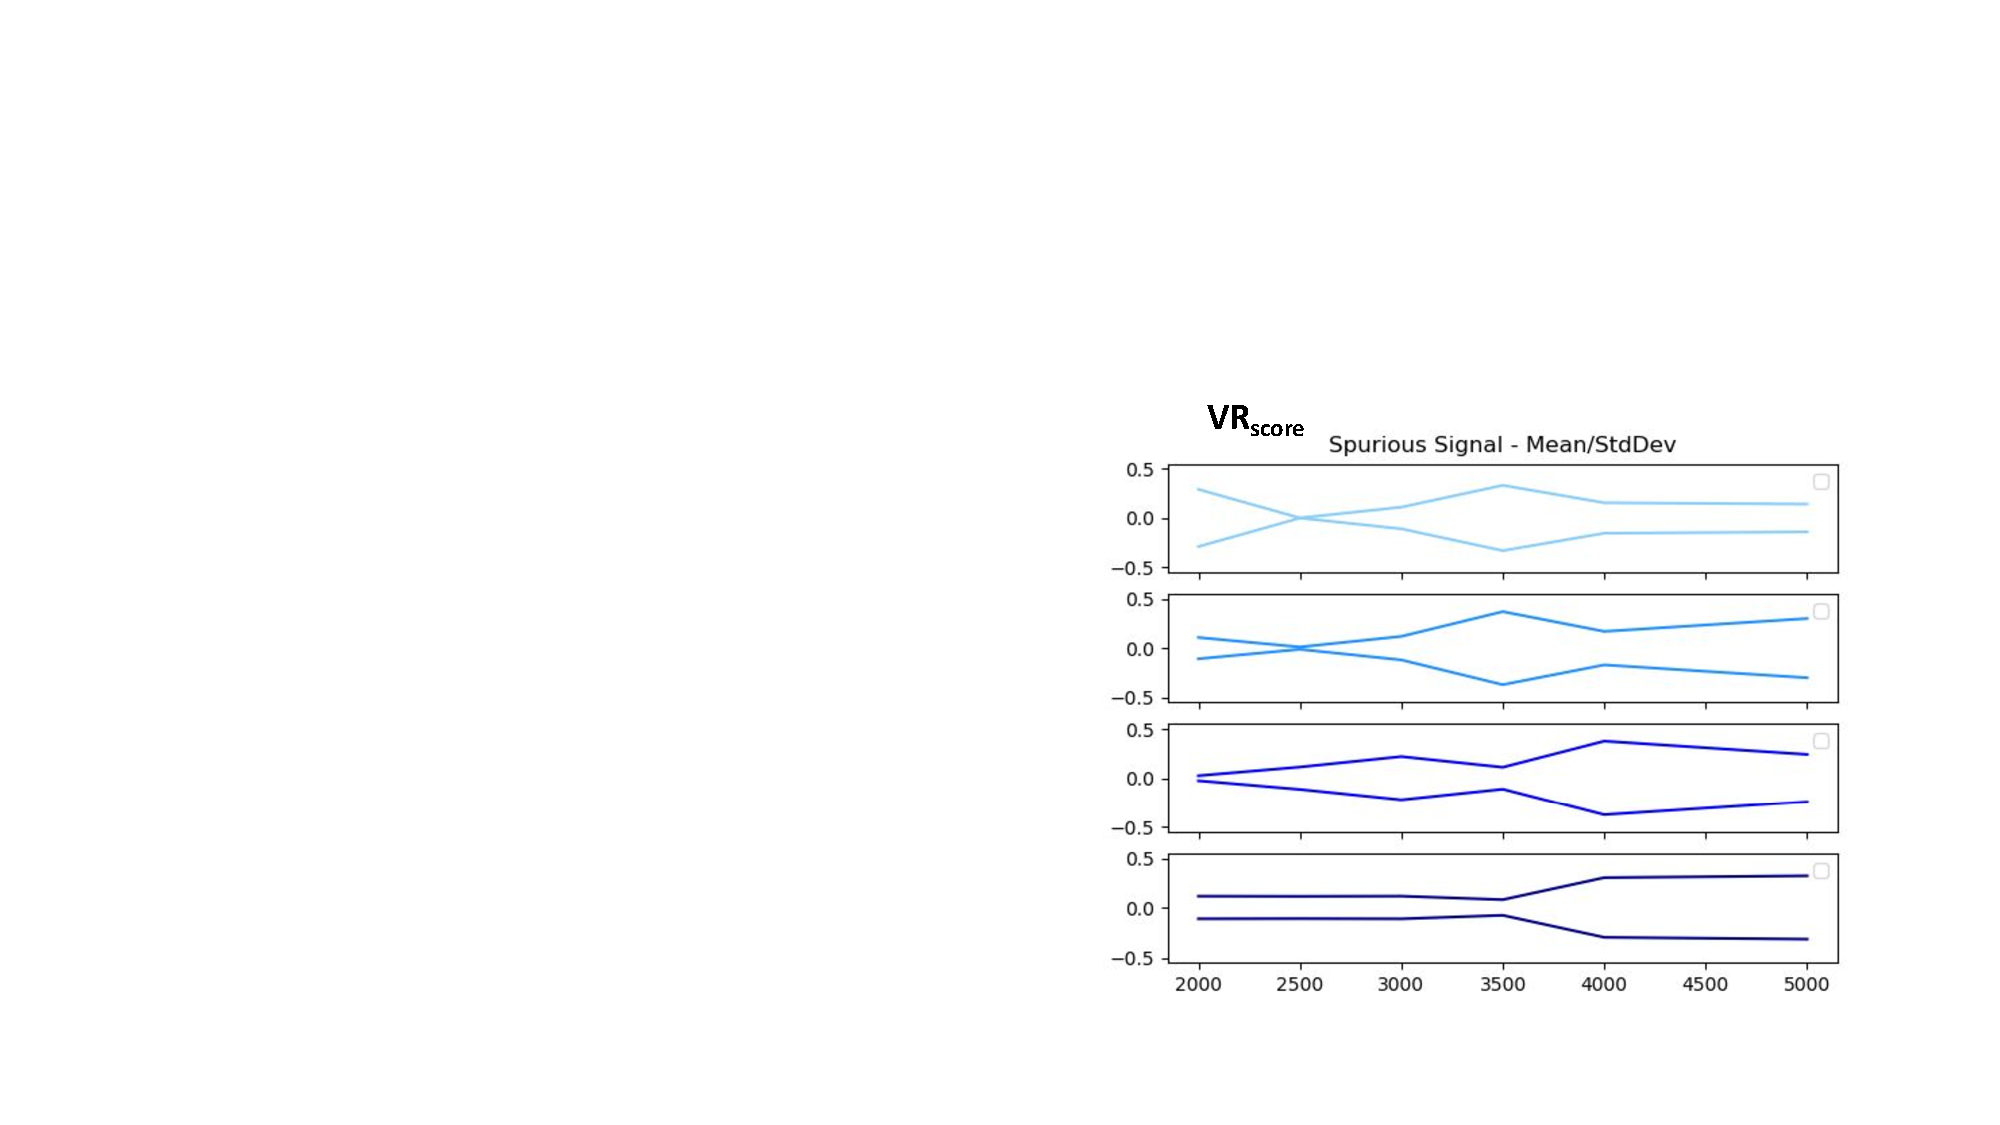
\includegraphics[width=0.6\textwidth]{figures/systs/spursig_vs_mass_vr}
    \caption{Fitted spurious signal in the VR, consistent with the CR and within the target size of $<$ 0.5 $\sigma$.
    \label{fig:spursig_vs_mass_vr}}
\end{figure}



%------------------------------------------------------------
\subsection{CP Variations}

Jet CP uncertainties are provided on the small-R jets, following the R22 Run 2 prescription~\cite{PERF-2014-07, PERF-2015-09, JETM-2018-05}.
They are implemented as \textit{shape} uncertainties on the signal samples in the statistical treatment.
There are 16 jet CP uncertainties available in the framework:

\begin{itemize}
  \item JET\_EtaIntercalibration\_NonClosure\_2018data
  \item JET\_EtaIntercalibration\_NonClosure\_highE
  \item JET\_EtaIntercalibration\_NonClosure\_negEta
  \item JET\_EtaIntercalibration\_NonClosure\_posEta
  \item JET\_Flavor\_Response
  \item JET\_GroupedNP\_1
  \item JET\_GroupedNP\_2
  \item JET\_GroupedNP\_3
  \item JET\_JER\_DataVsMC\_MC16
  \item JET\_JER\_EffectiveNP\_1
  \item JET\_JER\_EffectiveNP\_2
  \item JET\_JER\_EffectiveNP\_3
  \item JET\_JER\_EffectiveNP\_4
  \item JET\_JER\_EffectiveNP\_5
  \item JET\_JER\_EffectiveNP\_6
  \item JET\_JER\_EffectiveNP\_7restTerm
\end{itemize}

\begin{figure}[!htbp]
\centering
   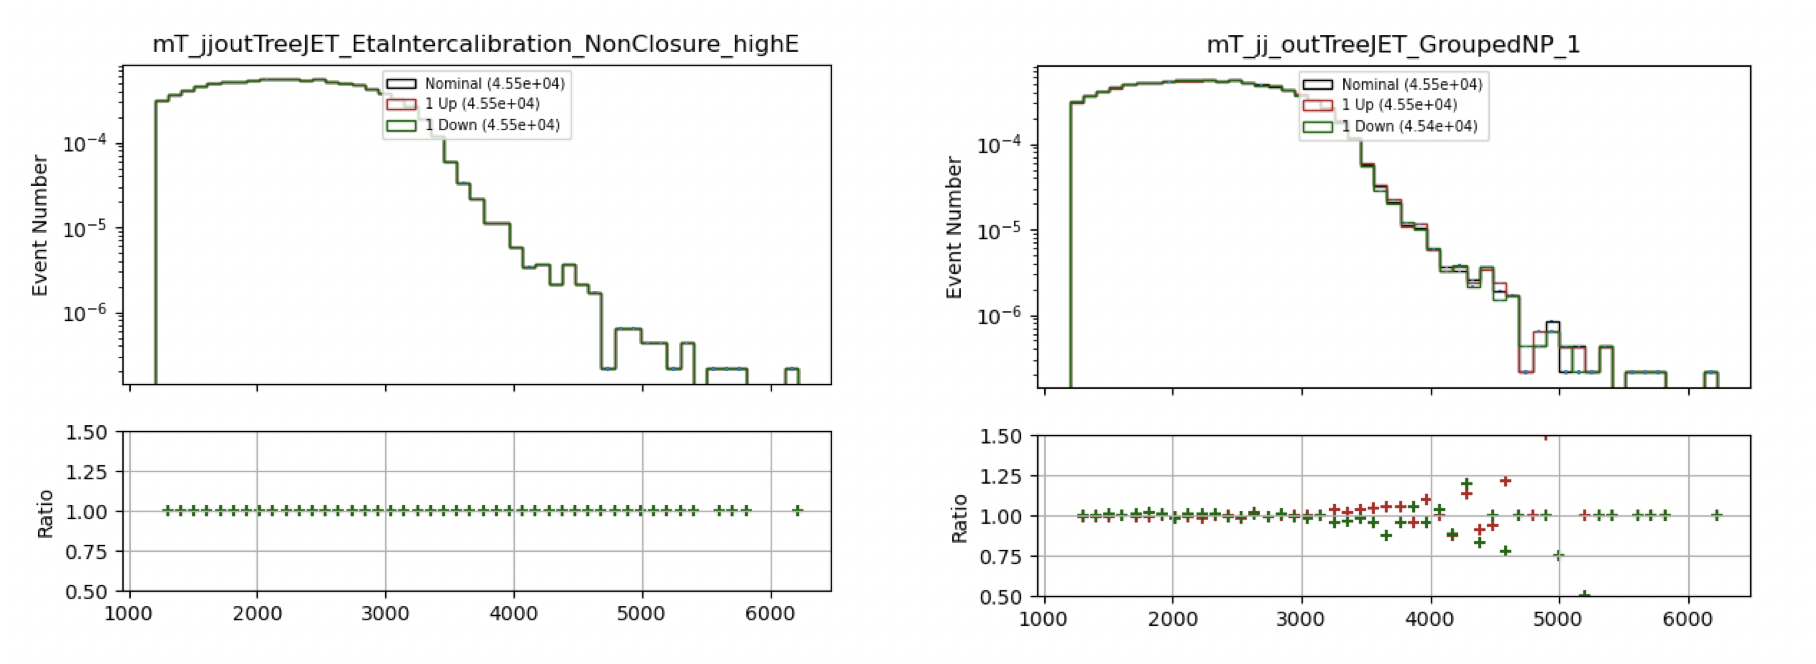
\includegraphics[width=0.85\textwidth]{figures/systs/jetCPshapes_1}
   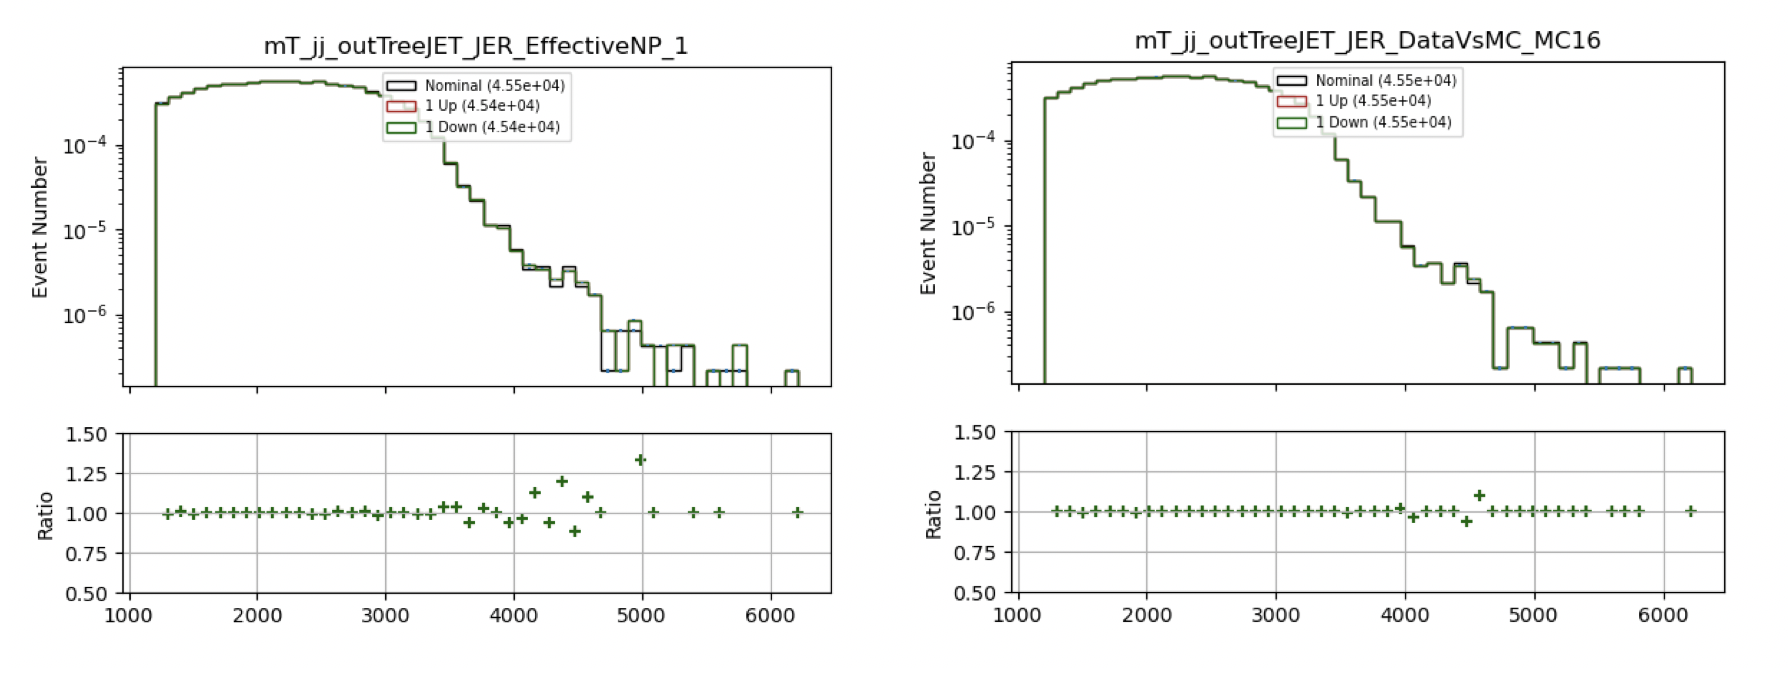
\includegraphics[width=0.85\textwidth]{figures/systs/jetCPshapes_2}
   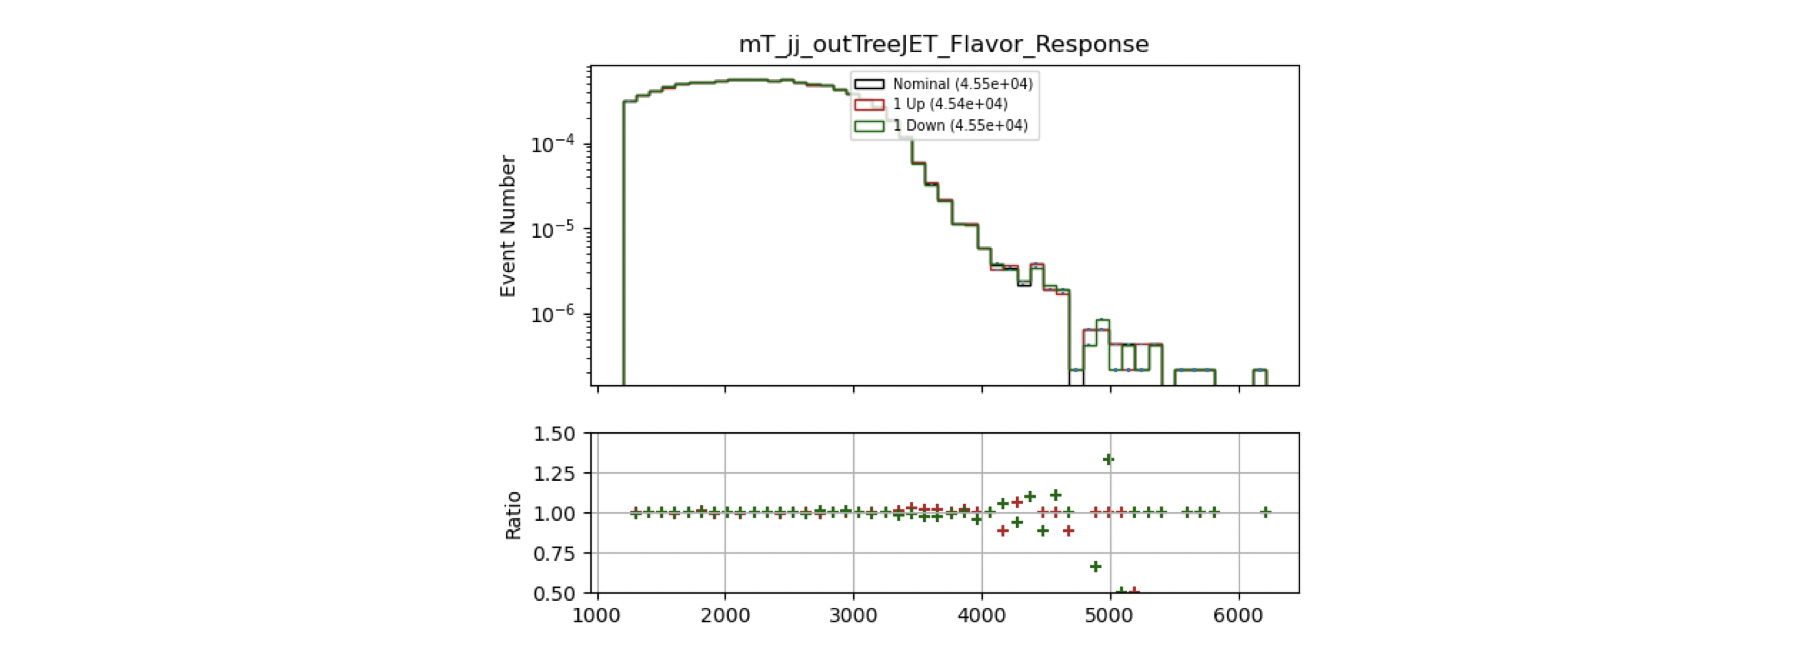
\includegraphics[width=0.85\textwidth]{figures/systs/jetCPshapes_3}
    \caption{Examples of the variation in the shape of mT in the SR due to various jetCP systematics.
    \label{fig:jetCPshapes}}
\end{figure}

\met~variations will also be studied before analysis approval.

\subsection{Theory Uncertainties}

The leading source of uncertainty on the theoretical signal model is the Pythia hadronization parameters, namely those that vary most significantly the number of dark hadrons in the shower.
These variations are evaluated to find the settings that yield the minimum and maximum number of dark hadrons, as recommended by Ref.~\cite{darkshowers_hadUncertainty}.
Figure~\ref{fig:pythiaHad} shows the impact of these variations on key analysis variables. 
These are preliminary results and will be followed up for the final interpretation.
\begin{figure}[!htbp]
\centering
   %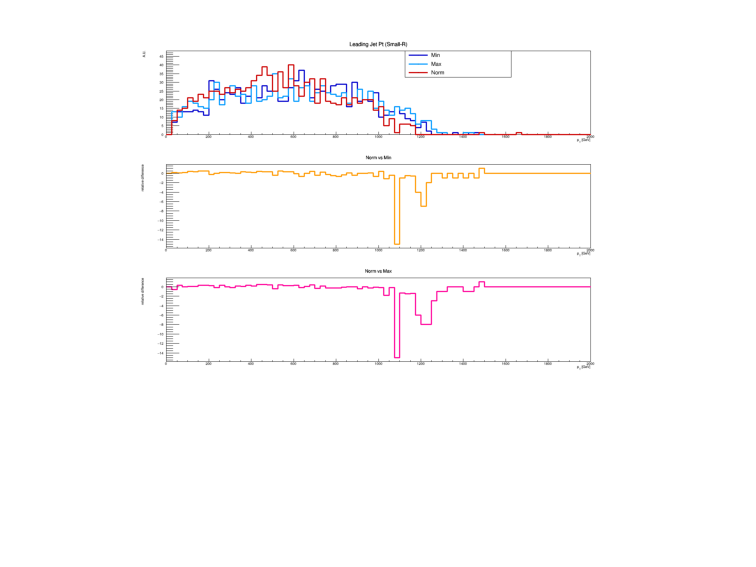
\includegraphics[width=0.5\textwidth]{figures/systs/pythiaHad_leadingjetpt}
   %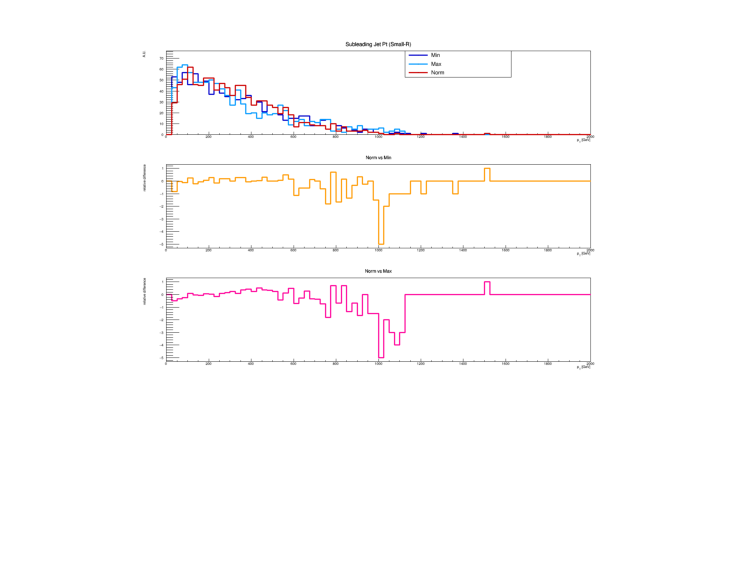
\includegraphics[width=0.5\textwidth]{figures/systs/pythiaHad_subleadingjetpt}
   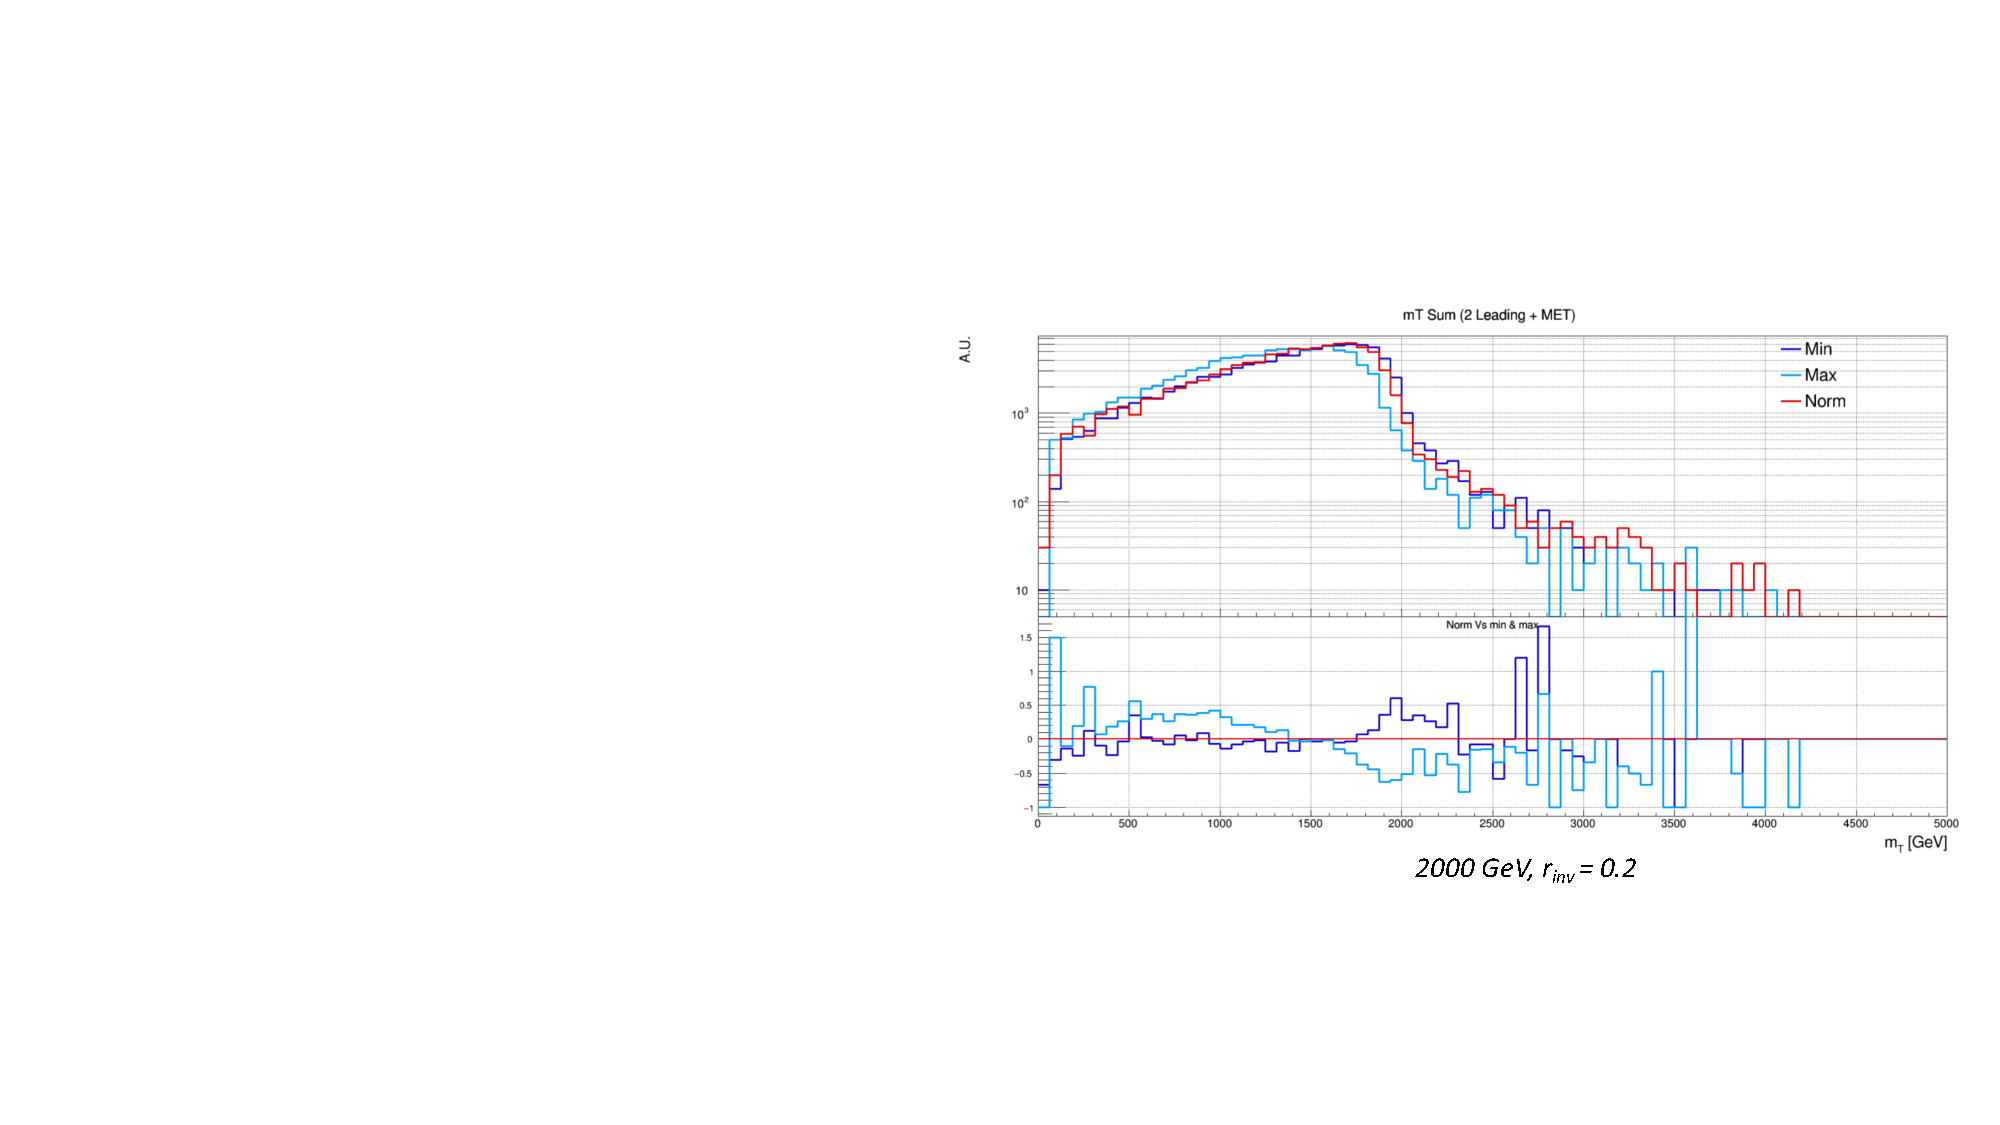
\includegraphics[width=0.6\textwidth]{figures/systs/pythiaHad_mT}
    \caption{Signal distribution of \mt, varying the Pythia hadronization parameters to produce the maximum/minimum number of dark hadrons.
    \label{fig:pythiaHad}}
\end{figure}

Signal theory uncertainties are also being considered, namely the value of $\alpha_s$ and ISR/FSR. 
Figure~\ref{fig:isrfsr} provides a look at the variations on the signal \mt~shape imposed by the standard prescription for measuring the ISR/FSR uncertainty~\footnote{\url{https://twiki.cern.ch/twiki/bin/view/AtlasProtected/MCTuningRecommendations}}.
These variations will be studied in greater detail and the most significant ones will be finalized and incorporated in final limits before approval.
\begin{figure}[!htbp]
\centering
   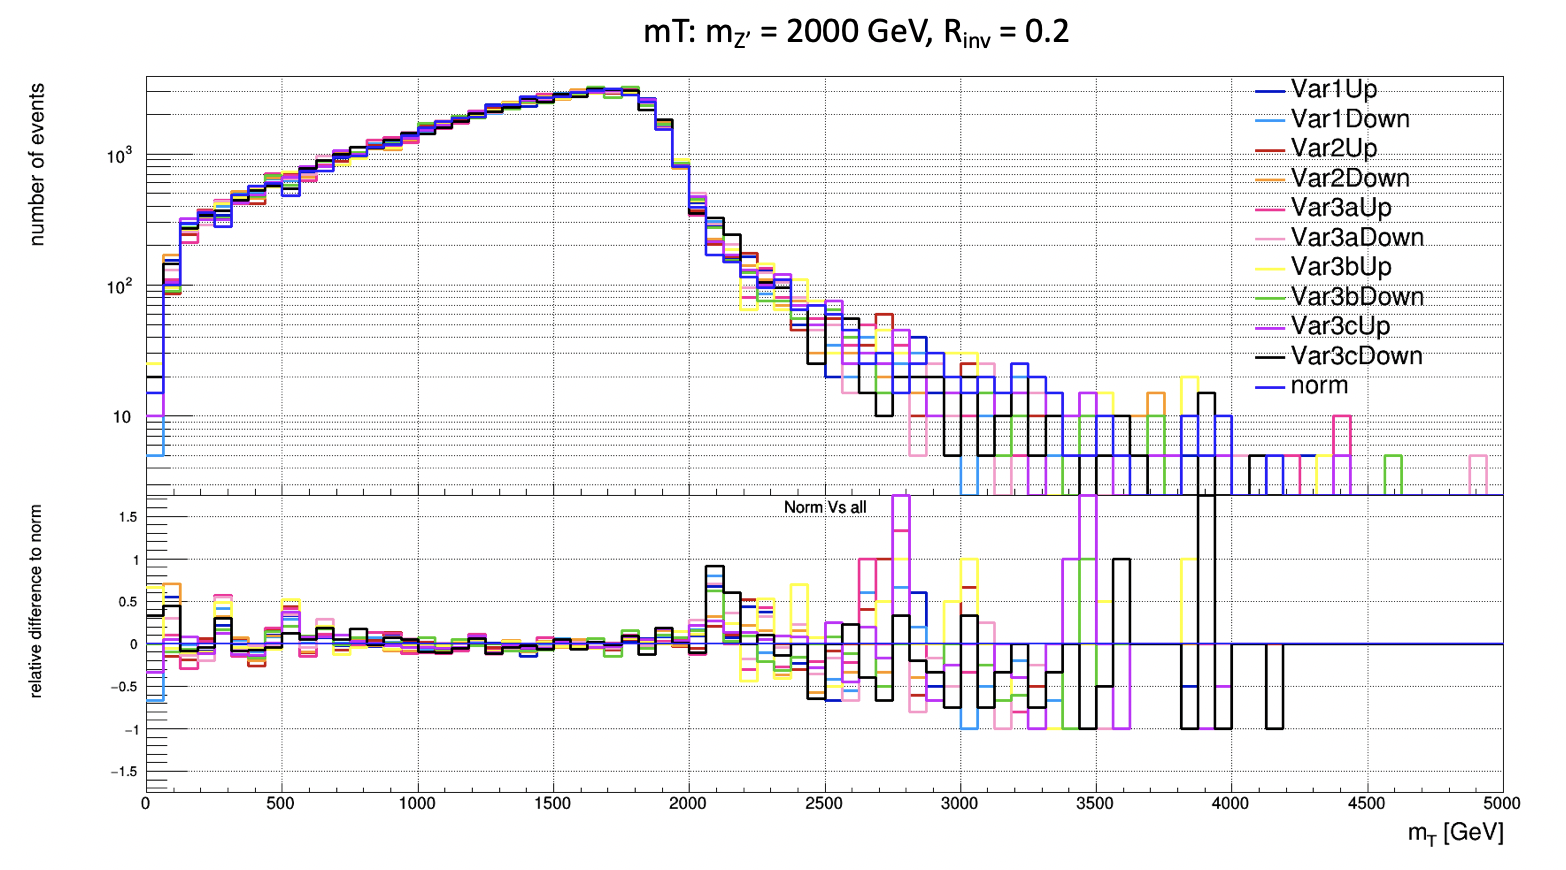
\includegraphics[width=0.7\textwidth]{figures/systs/isrfsr}
    \caption{Signal distribution of \mt, varying the ISR/FSR configuration.
    \label{fig:isrfsr}}
\end{figure}



\clearpage
